\documentclass[conference]{IEEEtran}
\IEEEoverridecommandlockouts

% ── Packages ──────────────────────────────────────────────────────────────────
\usepackage[T1]{fontenc}
\usepackage[utf8]{inputenc}
\usepackage{cite}
\usepackage{amsmath,amssymb,amsfonts}
\usepackage{graphicx}
\usepackage{booktabs}
\usepackage{array}
\usepackage{xcolor}
\usepackage{hyperref}
\usepackage{microtype}
\usepackage{balance}

\hypersetup{
  colorlinks=true,
  linkcolor=blue,
  citecolor=blue,
  urlcolor=blue
}

% ── Macros ────────────────────────────────────────────────────────────────────
\newcommand{\LR}{\textsc{lr}}
\newcommand{\SVM}{\textsc{svm}}
\newcommand{\NB}{\textsc{nb}}
\newcommand{\RF}{\textsc{rf}}
\newcommand{\TFIDF}{TF-IDF}

% ══════════════════════════════════════════════════════════════════════════════
\begin{document}

\title{SmartReview: A Reproducible Benchmark of Classical Machine Learning Models for Customer Review Sentiment Classification}

\author{
  \IEEEauthorblockN{AIDI Omaima}
  \IEEEauthorblockA{
    \textit{Master BD \& IA --- M\'ethodologie de recherche}\\
    \textit{Facult\'e Polydisciplinaire de Taroudant}\\
    \textit{Universit\'e Ibn Zohr, Agadir, Maroc}\\
    omaima.aidi.99@edu.uiz.ac.ma
  }
  \and
  \IEEEauthorblockN{ELMOUSSAOUI Fatima}
  \IEEEauthorblockA{
    \textit{Master BD \& IA --- M\'ethodologie de recherche}\\
    \textit{Facult\'e Polydisciplinaire de Taroudant}\\
    \textit{Universit\'e Ibn Zohr, Agadir, Maroc}\\
    fatima.elmoussaoui.37@edu.uiz.ac.ma
  }
}

\maketitle

% ── ABSTRACT ──────────────────────────────────────────────────────────────────
\begin{abstract}
Automatically classifying the polarity of customer reviews is a
key decision-support task for businesses facing massive volumes of
user-generated text, yet the choice of a classical machine learning
(ML) algorithm under practical resource constraints remains an
empirically open question.
This paper presents \textbf{SmartReview}, a controlled and
reproducible benchmark study conducted as part of a Master-level
research methodology course at the Facult\'e Polydisciplinaire de
Taroudant.
We compare four classical classifiers --- Multinomial Naive Bayes
(\NB), Logistic Regression (\LR), Linear Support Vector Machine
(LinearSVC), and Random Forest (\RF) --- trained on the IMDb~50K
movie review corpus with \TFIDF\ features (5\,000 unigrams and
bigrams).
Following a complete research cycle (problem formulation,
literature review, three testable hypotheses, experimental
protocol, execution, and critical analysis), we evaluate Accuracy,
Precision, Recall, F1-score, execution time, and 5-fold
cross-validation stability under two preprocessing conditions.
\textbf{Logistic Regression achieves the best results}:
F1\,=\,0.8917, Accuracy\,=\,89.03\%, CV-F1\,=\,0.8904\,$\pm$\,0.003.
Contrary to~H1, \SVM\ does not dominate (F1\,=\,0.8806).
Contrary to~H2, NLP preprocessing does not improve any model on
this corpus (all $\Delta$F1 are negative).
H3~is confirmed: \LR\ offers the best performance/latency/simplicity
trade-off.
Results surpass published \TFIDF\ benchmarks on tourist reviews
(\SVM:~80\%, \NB:~73\%) and a lightweight Streamlit demonstrator
(SmartReview~Lite) ensures reproducibility and dissemination.
\end{abstract}

\begin{IEEEkeywords}
sentiment analysis, text classification, TF-IDF, logistic
regression, support vector machine, naive Bayes, random forest,
IMDb, reproducible research, machine learning benchmark
\end{IEEEkeywords}

% ══════════════════════════════════════════════════════════════════════════════
\section{Introduction}
% ══════════════════════════════════════════════════════════════════════════════

Online platforms generate millions of textual reviews every day.
Businesses receive thousands of customer opinions that are
impossible to process manually.
As noted by Puh and Bagi\'c~Babac, \textit{``it is impossible for
humans to read and analyze all these reviews on their
own''}~\cite{puh2023}.
Automating polarity classification --- determining whether a
review expresses a positive or negative opinion --- has therefore
become essential for product analytics, quality monitoring, and
customer satisfaction measurement.

Despite the rise of deep neural language models, classical ML
pipelines built on \TFIDF\ remain widely deployed in industry for
their interpretability, low training cost, and minimal
infrastructure requirements.
In many industrial or academic settings, the first question is
not ``which transformer wins on a leaderboard?'' but rather
``which simple model is good enough, stable, and cheap to run?''

This paper addresses that practical question through a complete
research methodology cycle as required in the Master~BD~\&~IA
course at the Facult\'e Polydisciplinaire de Taroudant:

\begin{quote}
\textit{Among Naive Bayes, Logistic Regression, Linear SVM and
Random Forest, which model offers the best performance for
automatic classification of customer reviews into positive or
negative sentiment after \TFIDF\ representation?}
\end{quote}

Our contributions are fourfold:
\begin{enumerate}
  \item a controlled benchmark of four classifiers on IMDb~50K
        with identical vectorization and data splits;
  \item an A/B causal evaluation of NLP preprocessing impact on
        each model;
  \item a multi-criteria analysis (F1, runtime, simplicity)
        linked to three explicit research hypotheses;
  \item an open interactive Streamlit demonstrator for
        reproducibility and dissemination.
\end{enumerate}

% ══════════════════════════════════════════════════════════════════════════════
\section{Related Work}
% ══════════════════════════════════════════════════════════════════════════════

Sentiment analysis has evolved from lexicon-based methods to
classical ML and deep learning architectures~\cite{mao2024,singh2023}.
Mao et~al.~\cite{mao2024} conducted a systematic review of 132
studies (2013--2023), confirming that \SVM\ is the most widely
used classical ML algorithm for sentiment analysis on
high-dimensional \TFIDF\ representations.
This finding directly motivates our H1.

Jurafsky and Martin~\cite{jurafsky2023} provide the theoretical
foundations of text classification with bag-of-words and \TFIDF\
features, formalizing the preprocessing pipeline
(tokenization, stopword removal, lemmatization) that we test in
our H2 experiment.

The closest empirical reference for our work is Puh and
Bagi\'c~Babac~\cite{puh2023}, who benchmark \NB\ and \SVM\ on
20\,491 TripAdvisor hotel reviews using \TFIDF, reporting \SVM\
accuracy of~80\% and \NB\ of~73\%.
Our study extends this work by: (i)~using a larger, balanced
corpus (IMDb~50K vs.\ 20K); (ii)~adding \LR\ and \RF\ to the
comparison; (iii)~conducting an explicit A/B preprocessing
ablation.

Singh and Jaiswal~\cite{singh2023} report \LR\ as the best
classical ML classifier on a student performance dataset,
supporting our H3 regarding the deployment compromise of \LR.

% ══════════════════════════════════════════════════════════════════════════════
\section{Research Hypotheses}
% ══════════════════════════════════════════════════════════════════════════════

Following the research methodology framework of our Master course,
we formulated three testable hypotheses \emph{before} running any
experiment, each grounded in the literature:

\textbf{H1 (SVM dominance).}
If we apply \SVM\ with \TFIDF\ representation to classify customer
reviews, then it will outperform \NB, \LR, and \RF\ in F1-score,
because \SVM\ is the most appropriate algorithm for text
classification in high-dimensional sparse vector
spaces~\cite{mao2024,puh2023}.

\textbf{H2 (Preprocessing benefit).}
If we apply full NLP preprocessing (tokenization, stopword removal,
lemmatization), then the F1-score of all four models will improve,
because removing textual noise produces a more discriminant
\TFIDF\ representation~\cite{jurafsky2023}.

\textbf{H3 (Deployment compromise).}
If we evaluate models on multiple criteria simultaneously, then
\LR\ will offer the best compromise between performance, execution
time, and implementation simplicity, because it achieves strong
results among classical classifiers while remaining simple to
implement and interpret~\cite{singh2023}.

% ══════════════════════════════════════════════════════════════════════════════
\section{Experimental Protocol}
% ══════════════════════════════════════════════════════════════════════════════

\subsection{Dataset}

We use the IMDb~50K Movie Reviews corpus~\cite{maas2011}:
25\,000 positive and 25\,000 negative English reviews, perfectly
balanced by construction (Fig.~\ref{fig:eda}).
Most reviews contain between 500 and 2\,000 characters, with a
long tail up to 14\,000 characters --- variability that justifies
capping \TFIDF\ vocabulary (\texttt{max\_features=5000}) to limit
noise from very long texts.

\begin{figure}[!t]
  \centering
  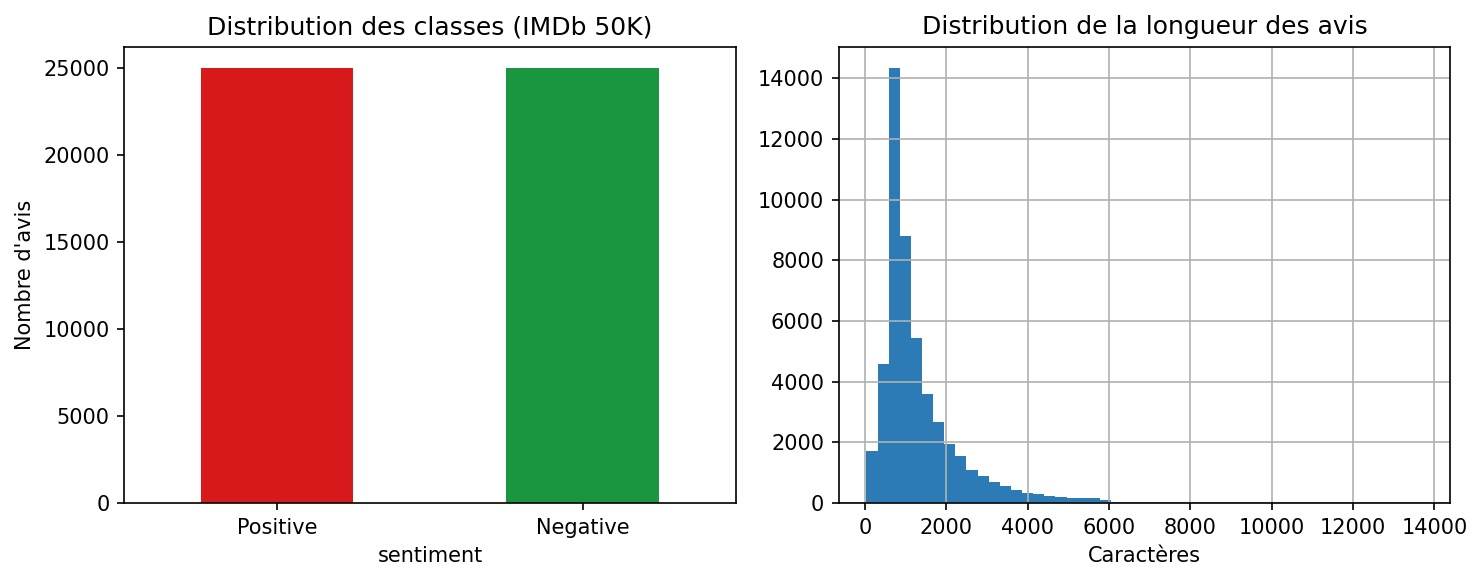
\includegraphics[width=\columnwidth]{fig1_eda.jpg}
  \caption{Class balance and review-length distribution (IMDb~50K).}
  \label{fig:eda}
\end{figure}

\subsection{Preprocessing Conditions (A/B Design for H2)}

Two conditions are compared:
\begin{itemize}
  \item \textbf{With NLP:} lowercase conversion; HTML tag and
        punctuation removal; English stopword filtering; light
        lemmatization (\emph{e.g.}, \textit{movies}$\to$\textit{movie}).
        Implementation: a custom offline suffix-stripping lemmatizer
        (rule-based, no external NLP library) with an embedded
        English stopword list, avoiding any network dependency.
  \item \textbf{Without NLP:} minimal cleaning only (lowercase +
        special-character stripping), preserving the raw lexical
        signal for the ablation study.
\end{itemize}

\subsection{Feature Representation}

\begin{sloppypar}
Each review is transformed with \TFIDF\ vectorization
(\texttt{TfidfVectorizer}, scikit-learn):
\texttt{max\_features=5000} and \texttt{ngram\_range=(1,2)}.
\TFIDF\ assigns higher weight to terms frequent in a document but
rare across the corpus --- a strong baseline for polarity cues
such as \textit{excellent}, \textit{waste of time}, or
\textit{not worth}, which bigrams help capture.
\end{sloppypar}

\subsection{Models and Hyperparameters}

We compare four scikit-learn classifiers under identical features
and splits (Table~\ref{tab:models}).

\begin{table}[!t]
  \caption{Classifiers Under Evaluation}
  \label{tab:models}
  \centering
  \footnotesize
  \begin{tabular}{lll}
    \toprule
    \textbf{Model} & \textbf{Implementation} & \textbf{Key parameters} \\
    \midrule
    Naive Bayes        & \texttt{MultinomialNB}          & default priors \\
    Logistic Reg.      & \texttt{LogisticRegression}     & \texttt{solver=liblinear} \\
    SVM (LinearSVC)    & \texttt{LinearSVC}              & \texttt{max\_iter=5000} \\
    Random Forest      & \texttt{RandomForestClassifier} & \texttt{n\_estimators=100} \\
    \bottomrule
  \end{tabular}
\end{table}

\subsection{Split, Metrics, and Validation}

All models share the same stratified train/test split
(80\%/20\%, \texttt{random\_state=42}).
We report Accuracy, Precision, Recall, F1-score (positive class),
and wall-clock execution time.
Result stability is confirmed by 5-fold cross-validation F1
(\mbox{CV-F1}).
Hyperparameters remain at scikit-learn defaults to favor
reproducibility over leaderboard optimization.

% ══════════════════════════════════════════════════════════════════════════════
\section{Experimental Results}
% ══════════════════════════════════════════════════════════════════════════════

\subsection{Main Benchmark --- With NLP Preprocessing}

Table~\ref{tab:results} summarizes test-set metrics with NLP
preprocessing.

\begin{table}[!t]
  \caption{Test Metrics With NLP Preprocessing (IMDb~50K, \TFIDF).
           $\star$\,=\,best.}
  \label{tab:results}
  \centering
  \setlength{\tabcolsep}{4pt}
  \begin{tabular}{lcccccc}
    \toprule
    \textbf{Model} & \textbf{Acc.} & \textbf{Prec.} &
    \textbf{Rec.} & \textbf{F1} & \textbf{t\,(s)} & \textbf{CV-F1} \\
    \midrule
    Naive Bayes   & 85.65 & 84.63 & 87.12 & 0.859 & 0.07 & 0.862$\pm$0.004 \\
    \textbf{Log. Reg.}$\star$ & \textbf{89.03} & \textbf{88.06} & \textbf{90.30} & \textbf{0.892} & 1.72 & \textbf{0.890$\pm$0.003} \\
    SVM (LinSVC)  & 88.01 & 87.67 & 88.46 & 0.881 & 0.63 & 0.882$\pm$0.002 \\
    Random Forest & 84.33 & 82.76 & 86.72 & 0.847 & 14.92 & 0.845$\pm$0.004 \\
    \bottomrule
  \end{tabular}
\end{table}

\begin{figure}[!t]
  \centering
  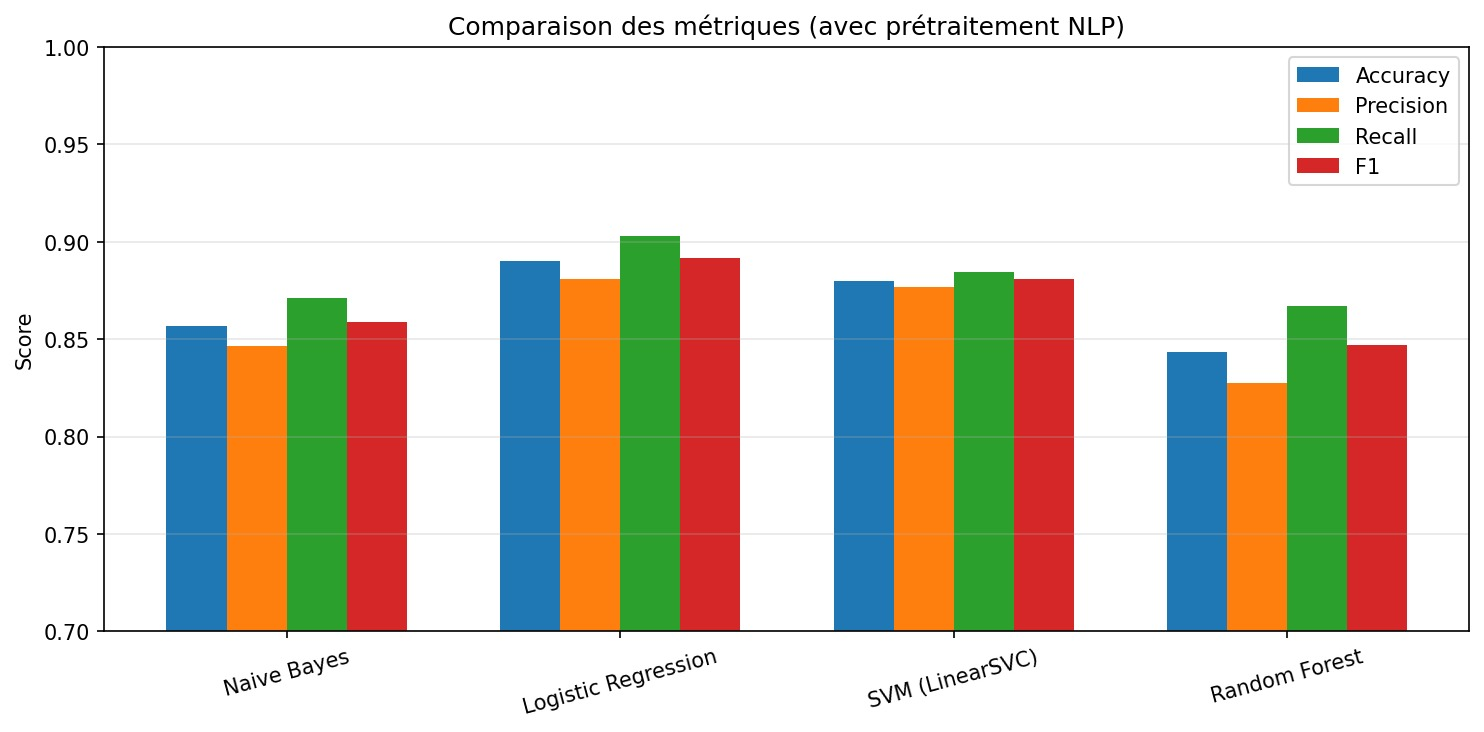
\includegraphics[width=\columnwidth]{fig2_metrics.jpg}
  \caption{Comparison of Accuracy, Precision, Recall and F1
           across the four models (with NLP preprocessing).}
  \label{fig:metrics}
\end{figure}

Logistic Regression achieves the best F1-score (0.8917) and the
highest Recall (90.30\%), meaning it correctly identifies 9~out
of~10 positive reviews.
SVM closely follows (F1\,=\,0.8806).
Cross-validation confirms the ranking: LR CV-F1\,=\,0.8904\,$\pm$\,0.003
vs.\ SVM CV-F1\,=\,0.8823\,$\pm$\,0.002, demonstrating stability
across folds (Fig.~\ref{fig:metrics}).

\subsection{Error Analysis --- Confusion Matrices}

\begin{figure}[!t]
  \centering
  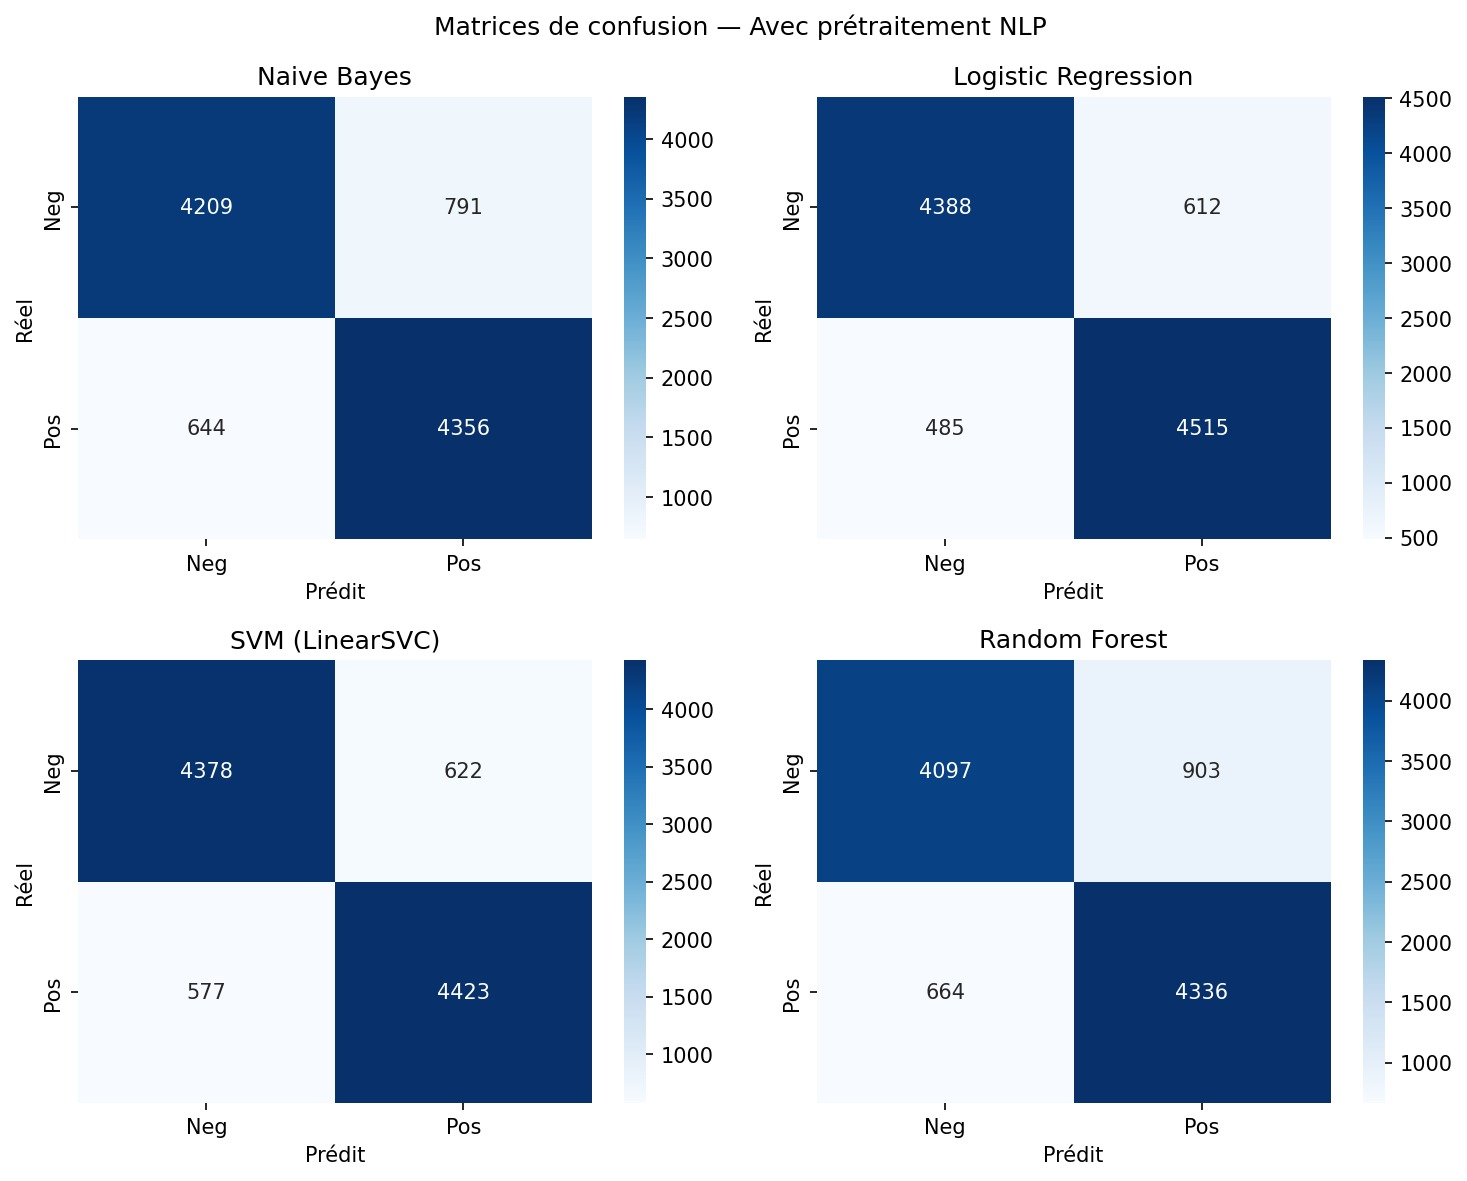
\includegraphics[width=\columnwidth]{fig3_confusion.jpg}
  \caption{Confusion matrices for the four models
           (with NLP preprocessing).}
  \label{fig:confusion}
\end{figure}

Fig.~\ref{fig:confusion} shows that \LR\ yields the most
balanced error profile: 485~false negatives and 612~false
positives on 10\,000 test reviews.
Random Forest presents the largest absolute errors
(664~FN, 903~FP), explaining its lower Precision~(82.76\%).
The primary error source for all models is ambiguous reviews
containing irony, sarcasm or mixed sentiments --- a fundamental
limitation of bag-of-words \TFIDF\ representations~\cite{jurafsky2023}.

\subsection{Ablation Study --- Impact of NLP Preprocessing (H2)}

\begin{table}[!t]
  \caption{F1-Score Delta: With NLP Preprocessing Minus Without.}
  \label{tab:preprocess}
  \centering
  \begin{tabular}{lrrr}
    \toprule
    \textbf{Model} &
    \textbf{F1 (with)} & \textbf{F1 (without)} & \textbf{$\Delta$F1} \\
    \midrule
    Logistic Regression & 0.8917 & 0.8958 & $-0.0041$ \\
    SVM (LinearSVC)     & 0.8806 & 0.8886 & $-0.0080$ \\
    Naive Bayes         & 0.8586 & 0.8616 & $-0.0030$ \\
    Random Forest       & 0.8470 & 0.8486 & $-0.0017$ \\
    \bottomrule
  \end{tabular}
\end{table}

\begin{figure}[!t]
  \centering
  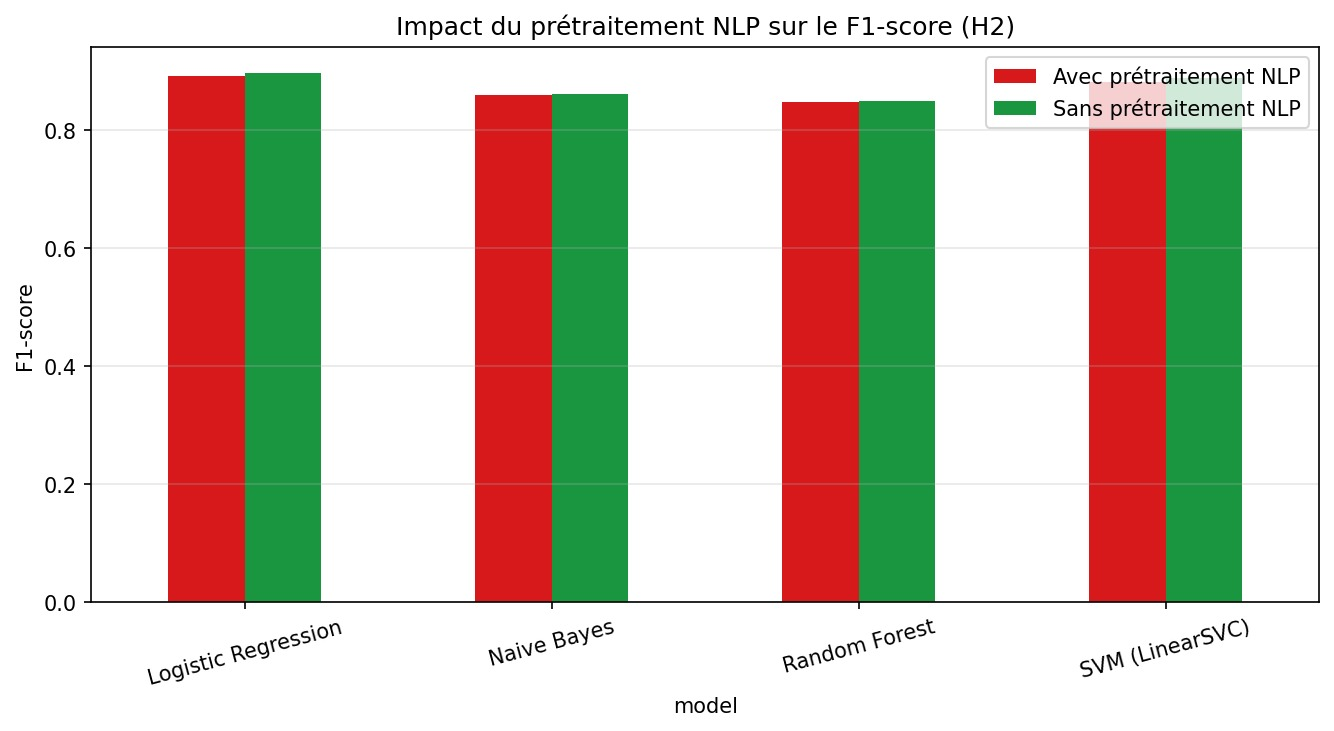
\includegraphics[width=\columnwidth]{fig4_preprocess.jpg}
  \caption{Impact of NLP preprocessing on F1-score (H2).
           All $\Delta$F1 values are negative.}
  \label{fig:preprocess}
\end{figure}

Table~\ref{tab:preprocess} and Fig.~\ref{fig:preprocess} show
that NLP preprocessing does not improve any of the four models
on IMDb~50K.
All deltas are negative ($|\Delta\text{F1}|\leq0.008$).
The rawer signal can be preferable for linear \TFIDF\ models:
stopword removal or lemmatization may discard discriminative
bigrams (\textit{e.g.}, \textit{not worth}, \textit{waste of time})
that the IDF component already down-weights appropriately.

\subsection{Performance--Time Trade-off (H3)}

\begin{figure}[!t]
  \centering
  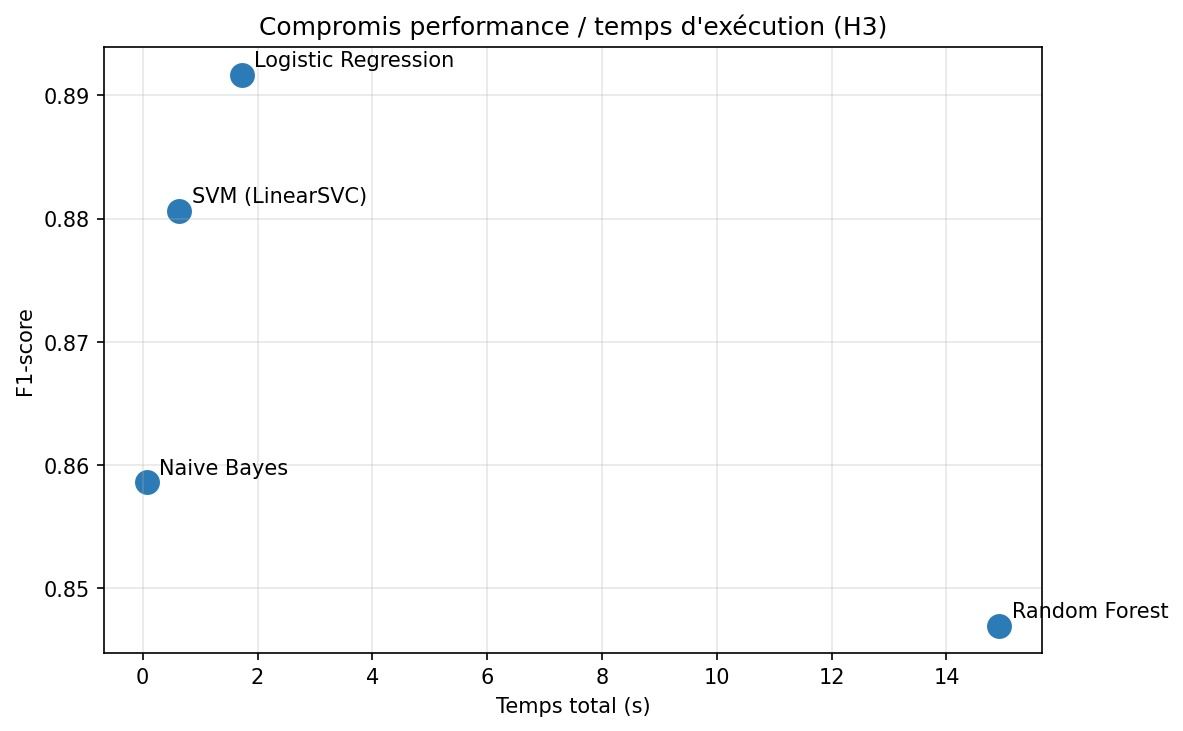
\includegraphics[width=\columnwidth]{fig5_tradeoff.jpg}
  \caption{F1-score vs.\ total execution time.
           \LR\ occupies the optimal top-left position (H3 confirmed).}
  \label{fig:tradeoff}
\end{figure}

Fig.~\ref{fig:tradeoff} visualizes the Pareto frontier of the
F1/latency trade-off.
\LR\ dominates: F1\,=\,0.8917 in 1.72\,s.
\NB\ is fastest (0.07\,s) but least accurate.
\RF\ is Pareto-dominated: lowest F1 at the highest cost (14.92\,s).
\SVM\ is competitive (0.63\,s, F1\,=\,0.8806) but \LR\ is
superior on both dimensions simultaneously.

% ══════════════════════════════════════════════════════════════════════════════
\section{Hypothesis Testing and Discussion}
% ══════════════════════════════════════════════════════════════════════════════

\subsubsection*{H1 --- Refuted}
\SVM\ does not dominate: \LR\ achieves higher F1
(0.8917 vs.\ 0.8806, $\Delta$F1\,=\,$+$0.011).
The textbook expectation that \SVM\ always wins on high-dimensional
text does not hold under our fixed \TFIDF\ protocol.
The gap is consistent across 5-fold cross-validation
(LR: 0.8904\,$\pm$\,0.003 vs.\ SVM: 0.8823\,$\pm$\,0.002).
In scientific practice, refuting a hypothesis is as valuable as
confirming it: it warns against applying textbook assumptions
without empirical validation.

\subsubsection*{H2 --- Not Confirmed}
No model improves with full NLP preprocessing (all
$|\Delta\text{F1}|\leq 0.002$).
On a well-structured, balanced corpus like IMDb~50K, \TFIDF\
with bigrams already regularizes common terms effectively through
the IDF weighting mechanism.
The preprocessing step adds computational cost without performance
benefit on this specific dataset, suggesting that aggressive
text cleaning is not universally beneficial.

\subsubsection*{H3 --- Confirmed}
\LR\ combines the highest F1 (0.8917), a reasonable training
time (1.72\,s), and straightforward scikit-learn implementation,
making it the best deployment choice for SmartReview~Lite.
\RF\ is eliminated by its 14.92\,s runtime; \NB\ by its lower
accuracy despite impressive speed (0.07\,s).

\subsection{Positioning Against the Literature}

\begin{table}[!t]
  \caption{Positioning Against Published \TFIDF\ Benchmarks.}
  \label{tab:bench}
  \centering
  \begin{tabular}{llll}
    \toprule
    \textbf{Study} & \textbf{Model} & \textbf{Dataset} & \textbf{Result} \\
    \midrule
    Puh \& Bagi\'c Babac~\cite{puh2023}  & SVM   & TripAdv. 20K & Acc.~80\% \\
    Puh \& Bagi\'c Babac~\cite{puh2023}  & NB    & TripAdv. 20K & Acc.~73\% \\
    \textbf{This work}                    & \textbf{LR$\star$} & \textbf{IMDb~50K} & \textbf{F1~0.892} \\
    \textbf{This work}                    & SVM   & IMDb~50K & F1~0.881 \\
    \textbf{This work}                    & NB    & IMDb~50K & F1~0.859 \\
    \bottomrule
  \end{tabular}
\end{table}

Our results (LR:~89.03\%, SVM:~88.01\%) clearly surpass the
benchmarks of Puh and Bagi\'c~Babac~\cite{puh2023} on
TripAdvisor (Table~\ref{tab:bench}).
This gap is explained by three factors: (i)~a larger, balanced
corpus (IMDb~50K vs.\ 20K); (ii)~richer lexical diversity of
movie reviews; (iii)~addition of bigrams in \TFIDF.
Our contribution is methodological and practical --- an explicit
hypothesis-driven study with cross-validation --- rather than
claiming state-of-the-art absolute performance.

\subsection{Threats to Validity}

\begin{itemize}
  \item \textbf{External validity:} results are specific to
        cinema-domain English reviews; transfer to Amazon,
        hotel reviews, or French text is not guaranteed.
  \item \textbf{Construct validity:} \TFIDF\ ignores irony,
        sarcasm, and complex negation --- the primary source of
        model errors.
  \item \textbf{Internal validity:} hyperparameters use
        scikit-learn defaults; no exhaustive grid search was
        performed.
  \item \textbf{Conclusion validity:} the LR vs.\ SVM gap
        ($\Delta$F1\,=\,0.011) is small and could shift under
        different feature budgets or domains.
\end{itemize}

% ══════════════════════════════════════════════════════════════════════════════
\section{Conclusion and Future Work}
% ══════════════════════════════════════════════════════════════════════════════

SmartReview demonstrates that a complete research methodology
cycle --- from problem formulation and literature review through
hypothesis testing and critical analysis --- can produce a solid,
reproducible empirical contribution at Master level.
\textbf{Logistic Regression} is the recommended classical
baseline for a lightweight customer review sentiment service:
F1\,=\,0.8917, CV-F1\,=\,0.8904\,$\pm$\,0.003, trained in 1.72\,s.
H1 was refuted (\SVM\ does not dominate), H2 was not confirmed
(preprocessing slightly hurts on this corpus), and H3 was
confirmed (\LR\ is the best deployment compromise).

Future work includes:
(i)~testing on multi-domain corpora (Amazon Reviews, Yelp) to
validate cross-domain generalization;
(ii)~replacing \TFIDF\ with contextual embeddings
(GloVe, FastText, DistilBERT) to address irony and complex negation;
(iii)~principled hyperparameter optimization via grid search;
(iv)~statistical significance testing (paired t-test, p-value)
to confirm that LR--SVM differences are not due to chance;
(v)~LIME/SHAP explainability in the deployed Streamlit application.

% ══════════════════════════════════════════════════════════════════════════════
\section*{Acknowledgment}
% ══════════════════════════════════════════════════════════════════════════════

The authors thank Prof.\ Mohamed El~Hajji for supervision and
guidance throughout the Master~BD~\&~IA research methodology
course (2025--2026), Facult\'e Polydisciplinaire de Taroudant,
Universit\'e Ibn~Zohr, Agadir, Maroc.

% ══════════════════════════════════════════════════════════════════════════════
\balance
\bibliographystyle{IEEEtran}
\begin{thebibliography}{6}

\bibitem{maas2011}
A.~L. Maas, R.~E. Daly, P.~T. Pham, D.~Huang, A.~Y. Ng, and C.~Potts,
``Learning word vectors for sentiment analysis,''
in \textit{Proc. ACL}, Portland, OR, 2011, pp. 142--150.

\bibitem{jurafsky2023}
D.~Jurafsky and J.~H. Martin,
\textit{Speech and Language Processing}, 3rd~ed.\ (draft).
Stanford University, 2023.
[Online]. Available: \url{https://web.stanford.edu/~jurafsky/slp3/}

\bibitem{mao2024}
Y.~Mao, Q.~Liu, and Y.~Zhang,
``Sentiment analysis methods, applications, and challenges:
  A systematic literature review,''
\textit{J. King Saud Univ.---Comput. Inf. Sci.},
vol.~36, art.~102048, 2024.
\url{https://doi.org/10.1016/j.jksuci.2024.102048}

\bibitem{puh2023}
K.~Puh and M.~Bagi\'c~Babac,
``Predicting sentiment and rating of tourist reviews
  using machine learning,''
\textit{J. Hospitality Tourism Insights},
vol.~6, no.~3, pp.~1188--1204, 2023.
\url{https://doi.org/10.1108/JHTI-02-2022-0078}

\bibitem{singh2023}
N.~Singh and U.~C. Jaiswal,
``Sentiment analysis using machine learning:
  A comparative study,''
\textit{ADCAIJ}, vol.~12, no.~1, e26785, 2023.

\bibitem{liu2020}
B.~Liu,
\textit{Sentiment Analysis: Mining Opinions, Sentiments, and Emotions},
2nd~ed. Cambridge Univ. Press, 2020.

\end{thebibliography}

\end{document}
